\section{A controlled laboratory: the linear chain with non-Gaussian noise}
\label{sec:experiments}

The linear chain of \cref{eq:linear} is the cleanest place to ask what structure is worth, because its
covariance is fixed by two numbers and everything beyond it by the noise law, and because its exact score is
available. We ask three things: what diffusion noise erases, and when (\cref{sec:theory}); whether the
kernel can be learned through that noise (\cref{sec:learning-results}); and what explicit structure buys
against networks (\cref{sec:buys}). Where it stops is \cref{sec:limits}. All comparisons use the frozen
configuration of \cref{app:protocol}: Laplace noise, $\corr=0.85$, $\nsites=32$, twelve log-spaced levels on
$[0.05,3]$, and the schedule-pooled relative score error against the tree-exact reference. Paired seeds are
the inferential unit, sixteen at the frozen configuration and eight in the sweeps across regimes; every
selection is made on development seeds or on a validation bundle that never enters a reported number.
Three information interfaces are distinguished throughout: (A) the standard denoising recipe, clean sequences
with a fresh corruption at every step; (B) clean sequences with one fixed corruption each; (C) one noised
view per sequence and nothing else, which is what EM--BP sees. Three reference points bracket every estimator
(\cref{app:oracles}): the isotropic score $-\vx$ at $\isoFloorLaplace$, the LMMSE oracle with the true
covariance at $\lmmseFloorLaplace$, the floor of every second-order estimator by \cref{prop:lmmse}, and the
exact score at zero.

\section{What survives diffusion noise: attenuation by statistical order}
\label{sec:theory}

Write $\gamma$ for the standard Gaussian on $\Reals^{\nsites}$, $\Hen{k}$ for the
probabilists' Hermite polynomials and $H_\nu(\vx)=\prod_i\Hen{\nu_i}(x_i)$ for their
products, of degree $|\nu|$. The channel \cref{eq:channel} acts on Hermite moments
diagonally.

\begin{theorem}[Hermite attenuation]
\label{thm:hermite}
For every multi-index $\nu$ with $\E_{\Pz}|\va|^{|\nu|}<\infty$,
$\;\E_{\Pt}[H_\nu(\vx_t)]=e^{-|\nu|t}\,\E_{\Pz}[H_\nu(\va)]$.
\end{theorem}
\begin{proof}
Mehler's identity $\E_{z}[\Hen{n}(\alpha a+\sqrt{1-\alpha^2}\,z)]=\alpha^n\Hen{n}(a)$ for
$z\sim\normal{0}{1}$ follows from the generating function
$e^{sx-s^2/2}=\sum_n\Hen{n}(x)s^n/n!$; coordinates are independent given $\va$, and
$\alpha=e^{-t}$.
\end{proof}
Nothing here requires $\Pz/\gamma\in L^2(\gamma)$---which fails for the Laplace chain and,
because $\lmax(\Sig_0)>2$, for the Gaussian chain at $\corr=0.85$---only finite moments.
Two consequences are exact at every $t$: cumulants of order $m\ge3$ scale as $e^{-mt}$
(Gaussian noise has none), and the degree-4 Hermite moments of two variance-matched laws
differ exactly by their fourth-cumulant tensors $\kfour$, attenuated by $e^{-4t}$.
Correlation lives at degree two and decays as $e^{-2t}$; non-Gaussian shape first appears
at degree four and decays as $e^{-4t}$. \emph{Diffusion noise is a low-pass filter on
statistical order.}

The consequence for scores and for learning is an expansion in the signal-to-noise
ratio $e^{-2t}$. Let $s=e^{-t}\vx/\Dt$, $b=e^{-2t}/\Dt$ and
$\Lambda(s,b)=\log\E_{\Pz}\exp(s\cdot\va-b|\va|^2/2)$, so that
$\log\Pt(\vx)=\log\gamma_{\Dt}(\vx)+\Lambda(s,b)$ and
$\score=-\vx/\Dt+(e^{-t}/\Dt)\nabla_s\Lambda$ exactly. Grading $\Lambda$ by order in
$e^{-t}$, its second-order part is the same for $\Pz$ and its covariance twin, and its
fourth-order part differs by a term linear in $\kfour$.

\begin{theorem}[Order-by-order information decay]
\label{thm:decay}
Let $\Pz$ have finite eighth moments and covariance $\Sig_0$, let $\Sgauss$ be the score
of its covariance twin, and let $\lmax=\lmax(\Sig_0)$. As $t\to\infty$,
\begin{align}
  \E_{\Pt}\lVert\score-\Sgauss\rVert^2
   &= \tfrac{1}{6}\Frob{\kfour}^2\,e^{-8t}\bigl(1+\epsilon_t\bigr),
  \label{eq:scoregap}\\
  I_t(\theta)&= \tfrac12\Frob{\partial_\theta\Sig_0}^2\,e^{-4t}\bigl(1+\epsilon_t\bigr)
  \ \ \text{if }\partial_\theta\Sig_0\neq0,
  \label{eq:info2}\\
  I_t(\theta)&= \tfrac1{24}\Frob{\partial_\theta\kfour}^2\,e^{-8t}\bigl(1+\epsilon_t\bigr)
  \ \ \text{if }\partial_\theta\Sig_0=0,\ \partial_\theta\kfour\neq0,
  \label{eq:info4}
\end{align}
with $\epsilon_t=O(e^{-2t}\lmax)$,
where $I_t(\theta)=\E_{\Pt}[(\partial_\theta\log\Pt)^2]$ is the Fisher information one
noised sequence carries about a parameter $\theta$ of $\Pz$, and $\Frob{\cdot}$ is the
Frobenius norm of the matrix or symmetric 4-tensor. For a Gaussian chain
\cref{eq:info2} is exact at every $t$ with
$I_t=\tfrac12\operatorname{tr}(\Sig_t^{-1}\partial_\theta\Sig_t\Sig_t^{-1}\partial_\theta\Sig_t)$.
\end{theorem}
The information statements \cref{eq:info2,eq:info4} are the diffusion-time form of a
principle established for low-SNR latent-variable models: the log-likelihood expands in
powers of the SNR with the order-$k$ term carrying $k$-th-moment information
\citep{katsevich2023likelihood,perry2019sample,bandeira2023estimation}, and Fisher
information about directions first identifiable at moment order $k$ scales as
$\mathrm{SNR}^k$ \citep{balanov2026gmm}; with $\mathrm{SNR}_t\simeq e^{-2t}$ these are
\cref{eq:info2,eq:info4}. The cumulant attenuation behind \cref{thm:hermite} is also
written down for the forward process by \citet{aarts2025cumulants}. What is new is
the score-level statement \cref{eq:scoregap} with its constant, made interpretable by
\cref{prop:lmmse}; the crossover below; and the exact verification and learning
consequences that follow. The proof (\cref{app:proofs}) expands $\Lambda$ to fourth order, takes the
$\gamma$-second moment of the leading Hermite term by Wick's theorem, and bounds the
remainder by the moment condition; the scalar leading term of \cref{eq:scoregap} is
$(\kfour/6)\Hen{3}(x)e^{-4t}$. The leading orders of a degree-2 and a degree-4 coordinate
do not couple, because $\Hen{2}$ and $\Hen{4}$ are $\gamma$-orthogonal, so the
\emph{efficient} information of a shape coordinate after the nuisance coordinates are
estimated has the same rate as its raw information.

\begin{remark}[General order]
The same grading gives, for a coordinate whose lowest non-vanishing Hermite footprint has
degree $m$, $I_t(\theta)\propto e^{-2mt}$: the leading term of $\partial_\theta\log\Pt$ is
$e^{-mt}$ times a degree-$m$ Hermite polynomial, whose $\gamma$-second moment is a
constant. The constants are explicit for $m=2,4$ above.
\end{remark}

\begin{corollary}[Sample complexity by order]
\label{cor:samples}
Estimating a covariance coordinate to fixed precision from sequences observed at level
$t$ needs $\nseq\propto e^{4t}$ of them; a shape coordinate needs $\nseq\propto e^{8t}$.
The ratio of the two informations is $\propto e^{-4t}$.
\end{corollary}

\paragraph{Where the asymptote begins.}
The expansion parameter is $e^{-2t}\lmax(\Sig_0)$, not $e^{-2t}$, with
$\lmax\le(1+\corr)/(1-\corr)$ for the chain. Below
$\tstar=\tfrac12\log\lmax(\Sig_0)$ the long-wavelength covariance modes are still of
order one and the rates are shallower; above it the exponents of \cref{thm:decay} hold.
At $\corr=0.85$, $\tstar=\gaussTstareightfive$: a strongly correlated chain keeps its
correlation information longer, and any measurement stopped near $\tstar$ sees slopes
short of $-4$ and $-8$.

\begin{figure*}[t]
  \centering
  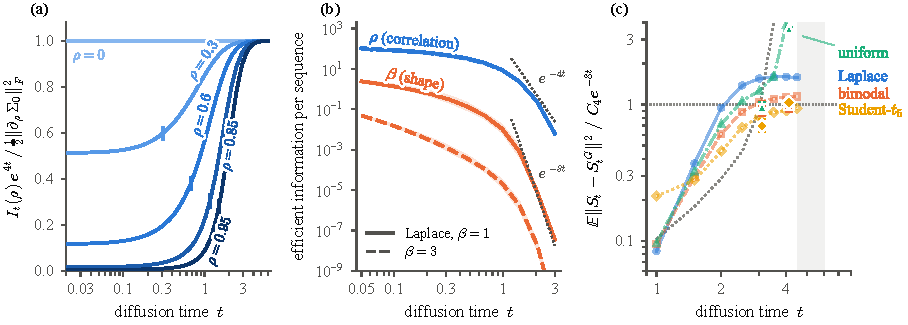
\includegraphics[width=\textwidth]{fig_theory.pdf}
  \caption{\textbf{What survives diffusion noise.}
  (a)~Exact Fisher information of the Gaussian chain about $\corr$, scaled by its
  predicted asymptote $\tfrac12\Frob{\partial_\corr\Sig_0}^2e^{-4t}$, for five $\corr$;
  every curve reaches~1, and the tick on each marks $\tstar(\corr)$.
  (b)~Efficient information per noised sequence about the correlation coordinate $\corr$
  (degree~2) and the shape coordinate $\beta$ (degree~4) of the generalised-Gaussian
  chain, from tree-exact inference and Fisher's identity, $\shapeChains$ sequences
  $\times\,\shapeReps$ replicates (bands: replicate range); guides $e^{-4t}$ and $e^{-8t}$.
  Above $\tstar$ the fitted slopes are $\shapeSlopeRhoone$ ($\corr$) and
  $\shapeSlopeBetathree$ ($\beta$, at $\beta=3$).
  (c)~The price of second-order closure: $\E\lVert\score-\Sgauss\rVert^2$ measured by
  tree-exact BP, divided by the predicted $\tfrac16\Frob{\kfour}^2e^{-8t}$, for four
  innovation families. Laplace and the bimodal mixture reach the constant to within
  $\closureRatiolaplacetthreepzero$--$\closureRatiobimodaltfourpzero$; Student-$t_5$, whose sixth
  moment is infinite, departs as the moment condition predicts; the uniform family reaches
  the floor of double precision near $t=3.5$.}
  \label{fig:theory}
\end{figure*}

\paragraph{Verification with the exact score.}
\Cref{fig:theory} tests \cref{thm:decay} where nothing has to be approximated. For the
Gaussian chain the closed form gives slope $\gaussSlopeRhoeightfive$ above $\tstar$ at
$\corr=0.85$ and the scaled information $\gaussScaledRhoeightfivetone$, $\gaussScaledRhoeightfivettwo$,
$\gaussScaledRhoeightfivetthree$ at $t=1,2,3$. For the non-Gaussian chain the shape information,
estimated from per-sequence scores obtained by Fisher's identity through the tree-exact
recursion, falls with slope $\shapeSlopeBetatwo$ ($\beta=2$) and $\shapeSlopeBetathree$
($\beta=3$) above $\tstar$, against the predicted $-8$, while the correlation
information falls with slope $\shapeSlopeRhotwo$ against $-4$; the kinked Laplace density
($\beta=1$) reaches the quadrature floor of the outer-product estimate near $t=2.5$.
The closure gap on the Laplace chain decays with slope $\closureSlopeSqlaplace$ and
reproduces the constant $\tfrac16\Frob{\kfour}^2$ ($\closureCfourlaplace$ for
$\nsites=32$) to $\closureRatiolaplacetthreepzero$ at $t=3$. The theorem also explains a
measurement the previous literature on this model reported as a discrepancy: information
slopes of about $-3$ and $-6$ obtained over $t\le1.6$ are the pre-asymptotic values below
$\tstar=\gaussTstareightfive$, not a failure of the $e^{-4t}$, $e^{-8t}$ law.

\paragraph{What this says about score learning.}
An estimator that carries only second-order structure cannot go below the LMMSE floor
$\lVert\score-\Sgauss\rVert$, which on the Laplace chain at $\corr=0.85$ is
$\lmmseFloorLaplace$ of the score energy pooled over the twelve-level schedule and
$\lmmseLowestLaplace$ at the lowest level (\cref{app:oracles}). A learner that recovers the
fourth-order structure has, by \cref{cor:samples}, $e^{4t}$ fewer effective samples per
sequence at level $t$ than one that recovers only covariance: the twelve-level schedule
is, for shape, effectively a four-level one. Both facts organise the experiments of
\cref{sec:experiments}.


\subsection{Learning the shape and the correlation through noise}
\label{sec:learning-results}

\paragraph{The information curve predicts what is learned at each level.}
\Cref{cor:samples} makes a prediction about learning that the exact score does not need: fitting from
$\nseq$ sequences all observed at level $t$, the shape of the driving-noise law stops being identifiable at
the level where its Cram\'er--Rao reference crosses the coordinate's range, while the correlation survives to
the crossover. This is also the arithmetic behind the one-view protocol: of twelve levels spread over
$t\in[0.05,3]$, only the lowest four carry appreciable information about shape.

\begin{figure}[t]
  \centering
  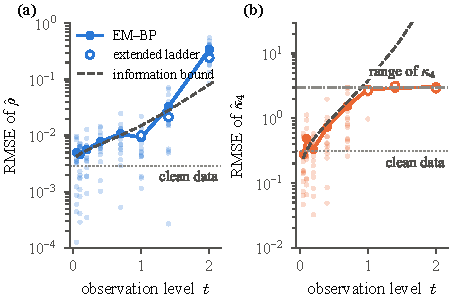
\includegraphics[width=\columnwidth]{fig_learning.pdf}
  \caption{\textbf{Learning through noise.} Recovery of the correlation coordinate and
  of the driving-noise shape from $\nseq=512$ sequences observed at a single level $t$,
  sixteen replicates (points: individual fits; line: RMSE), against the Cram\'er--Rao
  reference (dashed), the clean-data floor (dotted) and, for the shape, the coordinate's
  range. The fits are unimodal and at the reference at the lowest levels, split into a
  shrunk cluster and Gaussian-collapsed fits from $t=\learnLevelTzeropseven$, and collapse
  where the reference crosses the range. Hollow markers: the same fits with the \textsc{em}
  ladder extended to $\learnBudgetLadderMax$ iterations (\textsc{e06c}).}
  \label{fig:learning}
\end{figure}
%% Included by 04-learning.tex only when sections/learning-numbers.tex exists (E06 done).
\Cref{fig:learning} measures both with $\nseq=\learnSize$ Laplace-chain sequences and
$\learnSeeds$ replicates per level. Above $\tstar$ the fitted log-slopes of the two
errors against the observation level are $\learnSlopeRho$ for $\widehat\corr$ and
$\learnSlopeKurt$ for $\widehat\kfour$, against the predicted $2$ and $4$; their
difference, $\learnSlopeRatio$, is the $e^{2t}$ separation of \cref{cor:samples}. At
$t=0.1$ the fitted excess kurtosis is recovered to $\learnRmseKurtTzeropone$ RMSE and
the transition law to Hellinger distance $\learnHellTzeropone$; at $t=2$ the RMSE is
$\learnRmseKurtTtwo$ against a true value of $3$, while $\widehat\corr$ is still within
$\learnRmseRhoTtwo$. The clean-data fit (no channel) gives the optimiser's own floor,
$\learnRmseRhoTzero$ and $\learnRmseKurtTzero$.


\subsection{What explicit structure buys}
\label{sec:buys}

\paragraph{Capacity: the margin is fourth-order.}
%% Included by 05-experiments.tex only when sections/capacity-numbers.tex exists (E02a done).
%% GENERATED by tools/make_capacity_numbers.py from outputs/E02a -- do not hand-edit.
\begin{table}[t]\setlength{\tabcolsep}{4.5pt}
\centering
\small
\caption{Schedule-pooled relative score error on all sites, mean over $\capSeeds$ seeds (s.e.\ in the text macros; the isotropic reference is $\capIsoD$ at every size). Every arm is scored on identical test bundles. The last column is the same capacity fitted to the innovation law itself---the $\ncomp$-component mixture closest in Kullback--Leibler divergence, an infinite-data reference for the family rather than a bound; $\dagger$ marks fits whose narrowest component is under two grid cells.}
\label{tab:capacity}
\begin{tabular}{lcccc|c}
\toprule
& \multicolumn{4}{c|}{sequences $\nseq$} & \\
kernel & $32$ & $128$ & $512$ & $2048$ & $\nseq=\infty$ \\
\midrule
LMMSE floor & 0.167 & 0.167 & 0.167 & 0.167 & 0.167 \\
$\ncomp=1$ & 0.174 & 0.168 & 0.168 & 0.167 & 0.167 \\
$\ncomp=2$ & 0.084 & 0.050 & 0.035 & 0.028 & 0.039 \\
$\ncomp=4$ & 0.093 & 0.053 & 0.037 & 0.025 & 0.0057 \\
$\ncomp=8$ & 0.099 & 0.055 & 0.036 & 0.023 & 0.0022$^{\dagger}$ \\
$\ncomp=16$ & 0.100 & 0.056 & 0.036 & 0.022 & 0.0007$^{\dagger}$ \\
\bottomrule
\end{tabular}
\end{table}

\Cref{tab:capacity} places every arm on identical test bundles. A Gaussian-innovation
kernel ($\ncomp=1$) lands on the LMMSE floor at every size
($\capEmoneA$, $\capEmoneB$, $\capEmoneC$, $\capEmoneD$ against the floor
$\capLmmseA$--$\capLmmseD$), as \cref{prop:lmmse} requires; the mixture kernel goes
far below it, reaching $\capEmeightD$ at $\nseq=2048$, $\capFloorRatioD\times$ under the
floor. The paired $\ncomp=8$ versus $\ncomp=1$ difference is
$\capDiffD$ (bootstrap $[\capDiffDlo,\capDiffDhi]$) at $\nseq=2048$ and
$\capDiffA$ ($[\capDiffAlo,\capDiffAhi]$) already at $\nseq=32$, in favour of the
mixture in $\capWinsD$ and $\capWinsA$ of $\capSeeds$ seeds. The best capacity grows with
the data: $\ncomp=\capBestCapA$ at $\nseq=32$ and $\ncomp=\capBestCapD$ at
$\nseq=2048$, the usual variance-to-bias trade, and at $\nseq=2048$ the $\ncomp=8$ arm is
selected at the top of its iteration ladder in $\capAtCapeightD$ of $\capSeeds$ seeds, so
its error there is an upper bound on what a longer ladder would give. The fitted innovation
excess kurtosis is $\capKurteightD$ at $\nseq=2048$ against the true $3$; $\capUnresolved$
cells fail the two-grid-cell resolution gate and are reported, not dropped. The last row of
\cref{tab:capacity} is the family's infinite-data reference: the $\ncomp$-component mixture
closest in Kullback--Leibler divergence to the Laplace innovation, scored on the same
bundles. Its $\ncomp=1$ member is the covariance twin and scores $\capPopone$, the LMMSE
floor to three decimals, as \cref{prop:lmmse} requires; at $\ncomp=8$ it scores
$\capPopeight$, so the fitted kernel at $\nseq=2048$ sits $\capPopRatioeightD\times$ above
what its own family can express, a data limit rather than a capacity limit. (The reference is
not a bound: a Kullback--Leibler-optimal innovation need not minimise the score error, and
the $\ncomp=2$ fit at $\nseq=2048$ scores below it.)

An earlier study of this model concluded the opposite from a sweep that, it turned out, had fitted
every arm to a single training chain (\cref{app:capacity}); with independent chains and the checkpoint
selected identically for every capacity the effect is unambiguous.
Capacity buys exactly what the closure discards: across the generalised-Gaussian family at fixed
covariance the paired gain of $\ncomp=8$ over $\ncomp=1$ is ordered by $\kfour$,
$\famDiffBone$ at the Laplace member and a small loss, $\famDiffBtwo$, at the Gaussian
member, where there is no fourth-order structure to buy (\cref{app:family}, \cref{fig:family}).
The contrast is not a property of the frozen point: in all $\regCells$ cells of a sweep over
$\corr\in[\regRhoLo,\regRhoHi]$ and $\nsites\in[\regLenLo,\regLenHi]$ the mixture beats
the Gaussian kernel with the paired interval excluding zero, the paired difference
$\ncomp=8$ minus $\ncomp=1$ running from $\regGainStrongest$ at the most favourable corner
to $\regGainWeakest$ at the least, and in every cell the $\ncomp=1$
arm lands on the LMMSE floor to $\regIdentMax$, which checks the whole apparatus away from
the frozen configuration (\cref{app:regimes}).

\paragraph{Baselines under one recipe.}
%% Included by 05-experiments.tex only when sections/baseline-numbers.tex exists (E03 done).
%% GENERATED by tools/make_baseline_numbers.py -- do not hand-edit.
\begin{table*}[t]\centering\small\setlength{\tabcolsep}{4.5pt}
\caption{All-site schedule-pooled relative score error, mean over the confirmatory seeds ($\pm$ s.e.\ in the macros), every arm on identical test bundles. Oracles and EM--BP ($\ncomp=8$) from the capacity experiment; networks under the common recipe with the screened configuration.}
\label{tab:baselines}
\begin{tabular}{@{}rccccccccc@{}}
\toprule
$\nseq$ & isotropic & LMMSE & MLP & window & TCN & bi-GRU & transf. & U-Net & EM--BP \\
\midrule
32 & 0.669 & 0.167 & 0.517 & 0.186 & 0.223 & 0.201 & 0.231 & 0.227 & 0.099 \\
128 & 0.669 & 0.167 & 0.391 & 0.141 & 0.139 & 0.121 & 0.151 & 0.150 & 0.055 \\
512 & 0.669 & 0.167 & 0.276 & 0.121 & 0.096 & 0.078 & 0.097 & 0.095 & 0.036 \\
2048 & 0.669 & 0.167 & 0.208 & 0.118 & 0.068 & 0.060 & 0.063 & 0.066 & 0.023 \\
\bottomrule
\end{tabular}
\end{table*}

\Cref{tab:baselines} compares six architectures trained under one recipe (per-example noise
level, batch $64$, Adam with clipping, both output parameterisations, checkpoint selected on
validation), each with the configuration that won its family's screen on the development
seeds (\cref{tab:screen}, \cref{app:protocol}), on the test bundles of the capacity
experiment. Weight sharing is what separates the architectures at small $\nseq$: the fully
connected network reaches only $\baseWorstA$ at $\nseq=32$ against $\baseBestA$ for the
$\baseBestArchA$. Which shared architecture wins depends on the sample size---the
$\baseBestArchA$ at $\nseq=32$, the $\baseBestArchD$ at $\nseq=2048$---so locality is a
useful prior when sequences are scarce and a constraint when they are not.

Given enough clean sequences the networks pass the second-order floor: at $\nseq=2048$,
$\baseBelowFloorND$ of the six sit below $\baseLmmseD$ (\cref{prop:lmmse}), the best at
$\baseBestD$. They are not held at second order by anything intrinsic; they simply need the
data. The structured estimator is nonetheless ahead at every size---$\capEmeightD$ at
$\nseq=2048$, a paired factor $\baseRatioBestD$
($[\baseRatioBestDlo,\baseRatioBestDhi]$, favouring EM--BP in $\baseWinsBestD$ of
$\baseSeeds$ seeds) below the best network, and $\baseRatioBestA$ at $\nseq=32$---and it is
ahead while seeing strictly less of each sequence, which is what the next paragraph measures.

\paragraph{Information-matched training.}
Trained by implicit score matching on the one-view noisy bundle that EM--BP sees, with the
checkpoint selected on the implicit objective of a held-out noisy bundle and the true score
used only to report, the window head reaches $\matchedIsmoneviewWindowD$ and the transformer
$\matchedIsmoneviewTransformerD$ at $\nseq=2048$; with clean targets but a single fixed
corruption per sequence they reach $\matchedDsmonecorruptionWindowD$ and
$\matchedDsmonecorruptionTransformerD$. The distance between these and the standard-recipe
rows is the value of the clean signal and of fresh corruptions; the distance that remains to
EM--BP at the same interface is the value of the structure.

\paragraph{Length extrapolation.}
%% GENERATED by tools/make_baseline_numbers.py -- do not hand-edit.
\begin{table}[t]\centering\small\setlength{\tabcolsep}{4pt}
\caption{Length extrapolation at $\nseq=2048$: pooled relative score error of estimators fitted at $\nsites=32$ and evaluated against the tree-exact score of longer chains, mean over $\baseSeeds$ seeds. Longer chains are slightly easier (proportionally fewer boundary sites), so a length-agnostic arm should improve a little; the transformer instead breaks down beyond its training length.}
\label{tab:length}
\begin{tabular}{@{}lcccc@{}}
\toprule
arm & $\nsites=32$ & $\nsites=64$ & $\nsites=128$ & $\nsites=256$ \\
\midrule
bi-GRU & 0.060 & 0.057 & 0.057 & 0.056 \\
EM--BP & 0.023 & 0.023 & 0.023 & 0.023 \\
TCN & 0.068 & 0.066 & 0.065 & 0.064 \\
transf. & 0.063 & 0.243 & 0.514 & 0.703 \\
U-Net & 0.066 & 0.064 & 0.062 & 0.062 \\
window & 0.118 & 0.099 & 0.088 & 0.082 \\
\bottomrule
\end{tabular}
\end{table}

Fitted at $\nsites=32$ and evaluated at $\nsites=256$, the EM--BP kernel's error moves from
$\lenEmbpDLthreetwo$ to $\lenEmbpDLtwofivesix$: the learned law is local and the inference is
exact at any length. The window head, also local, moves from $\lenWindowDLthreetwo$ to
$\lenWindowDLtwofivesix$; the transformer with relative positions from
$\lenTransformerDLthreetwo$ to $\lenTransformerDLtwofivesix$ (\cref{tab:length}).


\begin{figure*}[t]
  \centering
  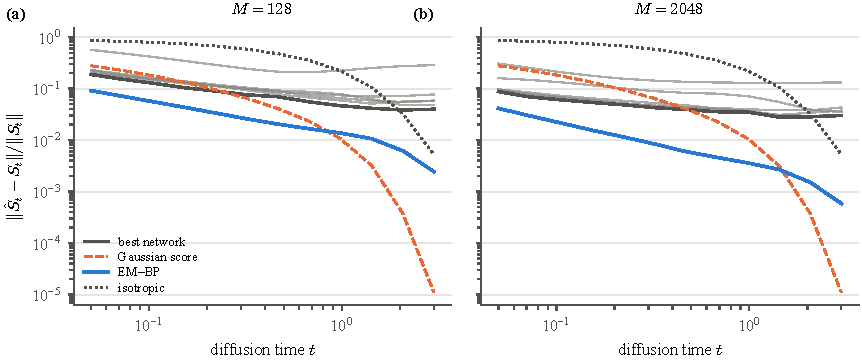
\includegraphics[width=\textwidth]{ff-nongaussian-gain.pdf}
  \caption{\textbf{Where the gain is.} Per-level relative score error against the exact score on the
  linear chain with Laplace noise, for $\nseq=128$ (a) and $\nseq=2048$ (b) training sequences: EM--BP
  (blue), the best of the six networks (thick grey; the other five thin), the Gaussian
  score (dashed) and the isotropic score (dotted). EM--BP is the best estimator at the lowest
  $\lvlFirstLevelsA$ (a) and $\lvlFirstLevelsB$ (b) of twelve levels. The Gaussian score, which is given the true
  covariance, overtakes it from $t=\lvlCrossA$ (a) and $t=\lvlCrossB$ (b) upward (the first level at which it is better,
  median over seeds), because nothing non-Gaussian is left to recover; no network is first at any level.}
  \label{fig:gain}
\end{figure*}

\begin{figure*}[t]
  \centering
  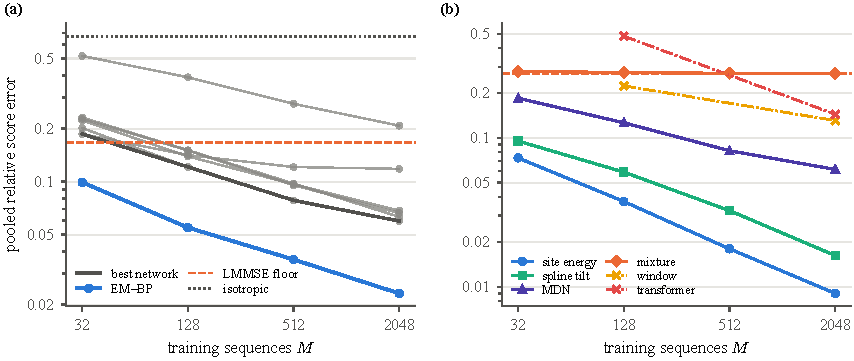
\includegraphics[width=\textwidth]{ff-sample-efficiency.pdf}
  \caption{\textbf{Sample efficiency.} Pooled relative score error against the number of training
  sequences. (a)~The linear chain with Laplace noise: EM--BP ($\ncomp=8$), the six networks (best in dark
  grey) and the LMMSE floor (dashed). (b)~The $\phi^4$ field at $\Temp=0.3$, $\latt=1$: the site energy, a
  spline-tilted kernel, an MDN kernel, the paper's mixture kernel and two networks, against the field's
  linear floor (dashed).}
  \label{fig:efficiency}
\end{figure*}

\paragraph{Generation.}
%% Included by 05-experiments.tex only when sections/generation-numbers.tex exists (E05 done).
Samples are drawn by the same reverse SDE (\genSteps{} steps on a geometric grid, one
Brownian path shared by every arm, \genSeeds{} seeds) from the exact score, the fitted
kernel, the LMMSE twin and the isotropic score, and compared with a reference sample of
the true law at $t_{\min}$ (\cref{tab:generation}). The exact arm's log-likelihood gap,
$\genLoglikgapDExact$ nats per sequence at $\nseq=2048$, is the sampler's own discretisation
error, the reference against which the other arms are read; the fitted kernel sits at $\genLoglikgapDEm$, the LMMSE twin at
$\genLoglikgapDLmmse$ and the isotropic score at $\genLoglikgapDIso$. The excess kurtosis of the
generated sequences' autoregressive residuals at $t_{\min}$, where the residual noise
lowers even the true law's value below the innovation's $3$, is $\genKurtgenDEm$ for the
fitted kernel against $\genKurtrefD$ for the true law and $\genKurtgenDLmmse$ for the twin, which by
construction generates Gaussian innovations: what the second-order estimator discards in
score error it discards in the samples.

Because the kernel is known after learning, generation does not need the reverse process at all: one
forward sweep from the learned kernel draws a sequence, and with the true kernel it samples at the Monte
Carlo floor of exact draws while costing $\genAncestralCostRatio\times$ less than a $200$-step reverse SDE
(\cref{app:tables}). A Gaussian score generates Gaussian sequences, whatever its accuracy at second order.

